\documentclass[]{article}
\usepackage{caption,subcaption,graphicx,float}
\graphicspath{{figs/}} 
%opening
\title{Notes from Origins of Life}
\author{}

\begin{document}

\maketitle


\begin{abstract}
    This course aims to push the field of Origins of Life research forward by bringing new and synthetic thinking to the question of how life emerged from an abiotic world.

\end{abstract}

\tableofcontents
\listoffigures

\section{Introduction}
\subsection{Welcome To The Course}
\subsection{Life}
\cite{bell2015potentially}
\subsection{Nonequilibrium Physics}
\subsection{Constraining Chemical Complexity to Form Life}
\subsection{Geological Conditions, Change, and Chaos}
\subsection{Pattern Formation in Chemical Systems}
\subsection{The Central Dogma of Biology}
\cite{crick1958biological} \cite{crick1970central}
\subsection{Biological Similarity}
\subsection{Selection Theory}
\cite{eigen1978hypercycle} \cite{eigen1988molecular} \cite{eigen2002error} \cite{crotty2001rna} \cite{stadtler2002fitness_landscapes}
\section{Chemical Origins}
\subsection{Introduction}

We will discuss likely chemistry of the early Earth, chemistry that may be to be fundamental to the origin of life, what we know is essential for biochemistry of modern life, processes that can occur in chemical dynamics, and extreme life that occurs today in a variety of environments.


\subsection{What Did Early Earth Look Like?}

\subsubsection{Geochemical Landscape}
\begin{figure}[h!]
	\caption{Geochemical Landscape after \cite{kitadai2018origins}}
	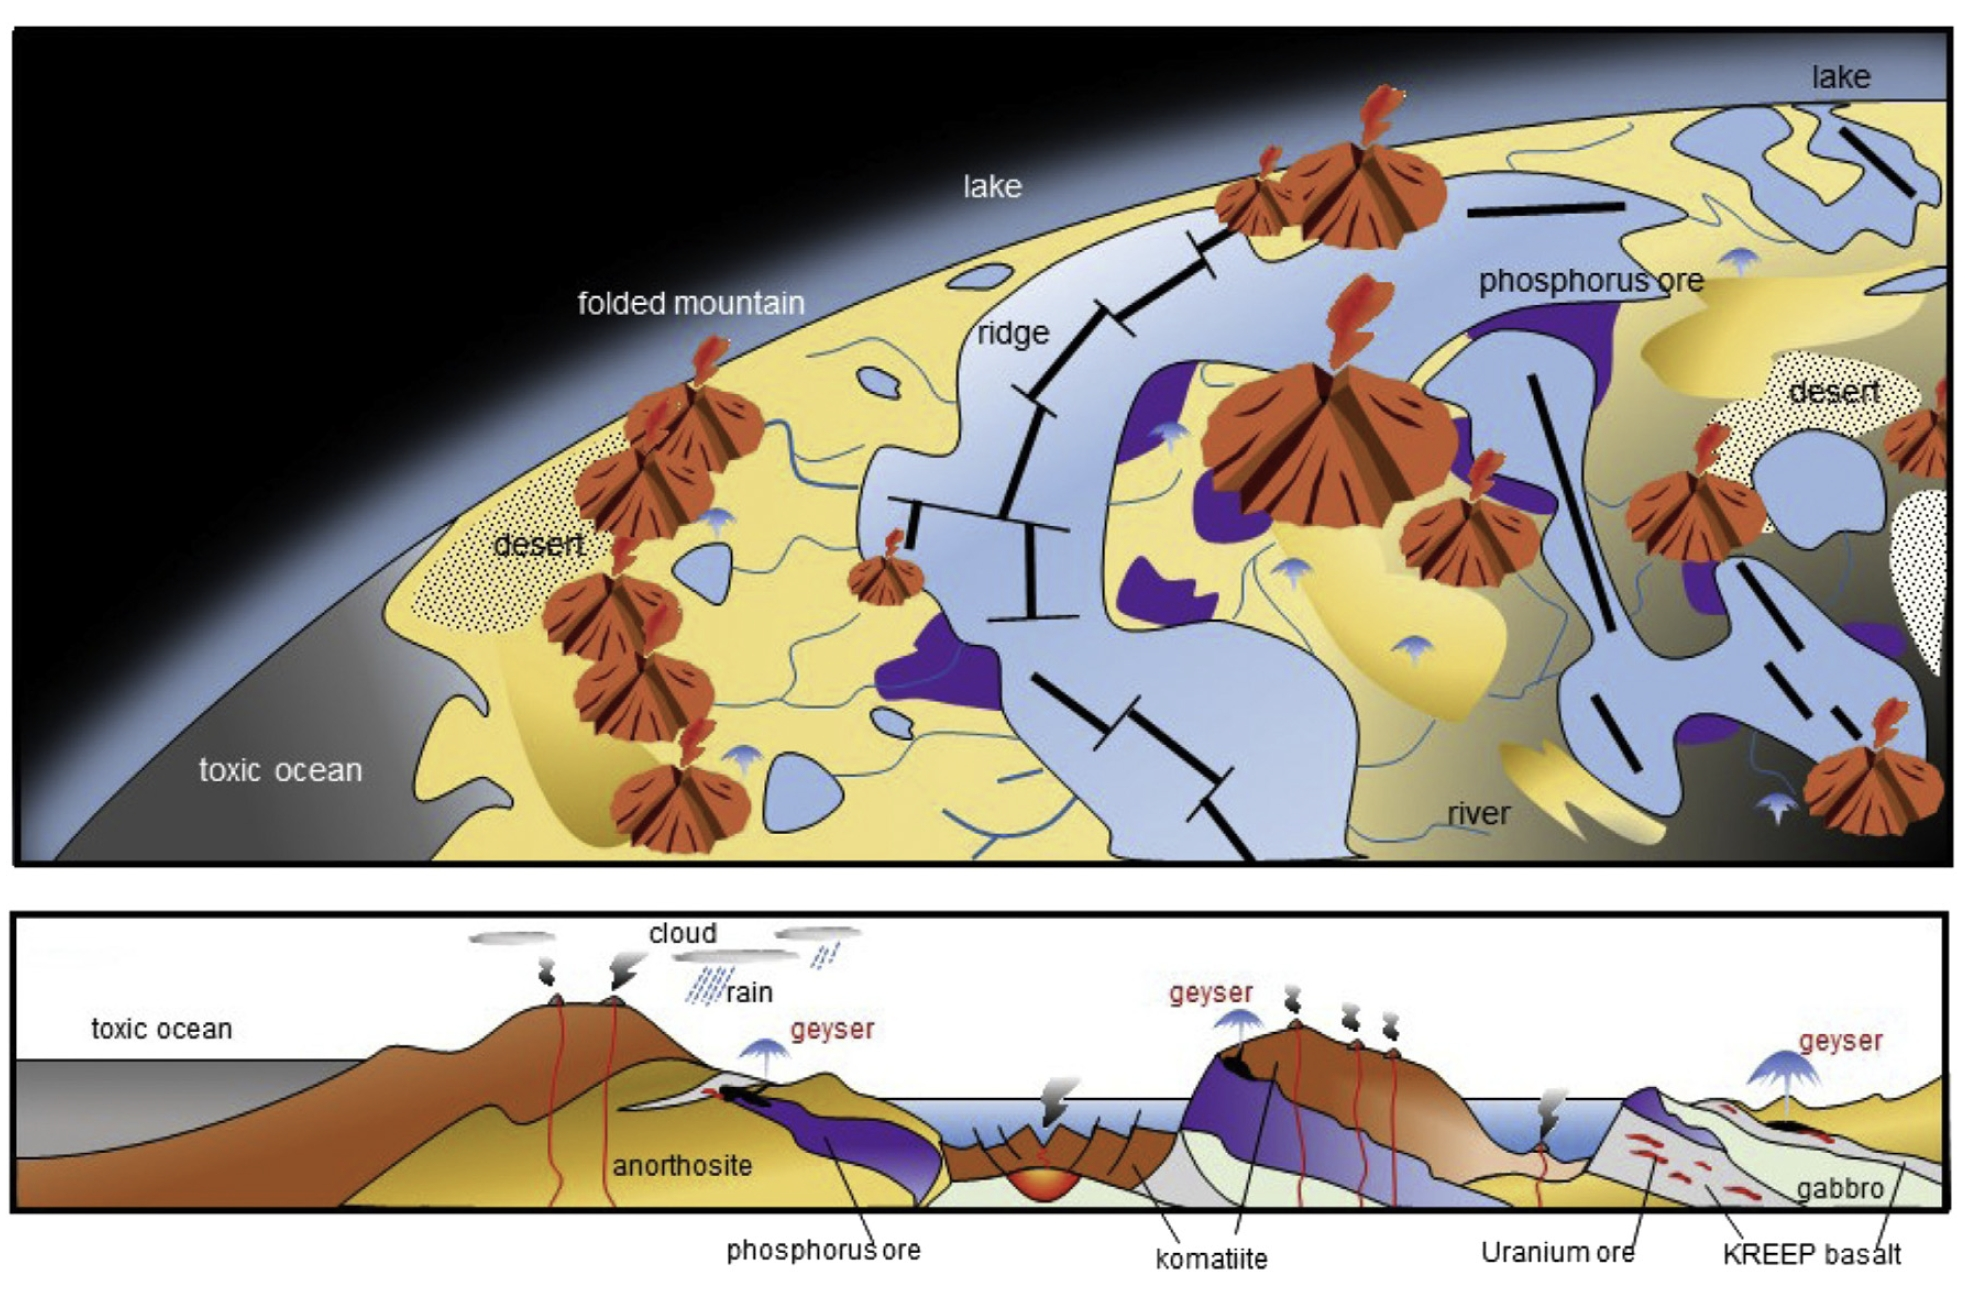
\includegraphics[width=0.9\textwidth]{GeochemicalLandscape}
\end{figure}

  
  \begin{itemize}
  	\item  Definitely an ocean that was warmer than today, probably saltier.
  	\item Landmasses from volcanic activity, and, maybe, plate tectonics.
  	\item On continents, lakes and ponds from precipitation.  Maybe temporary streams from precipitation.
  	\item Surfaces composed of minerals, which were good for catalysis and energy production. Today covered with life.
  \end{itemize}


\subsubsection{Mixing processes between chemical reactors}
\begin{figure}[h!]
	\caption{Mixing processes between chemical reactors \cite{stueken2013did}}
	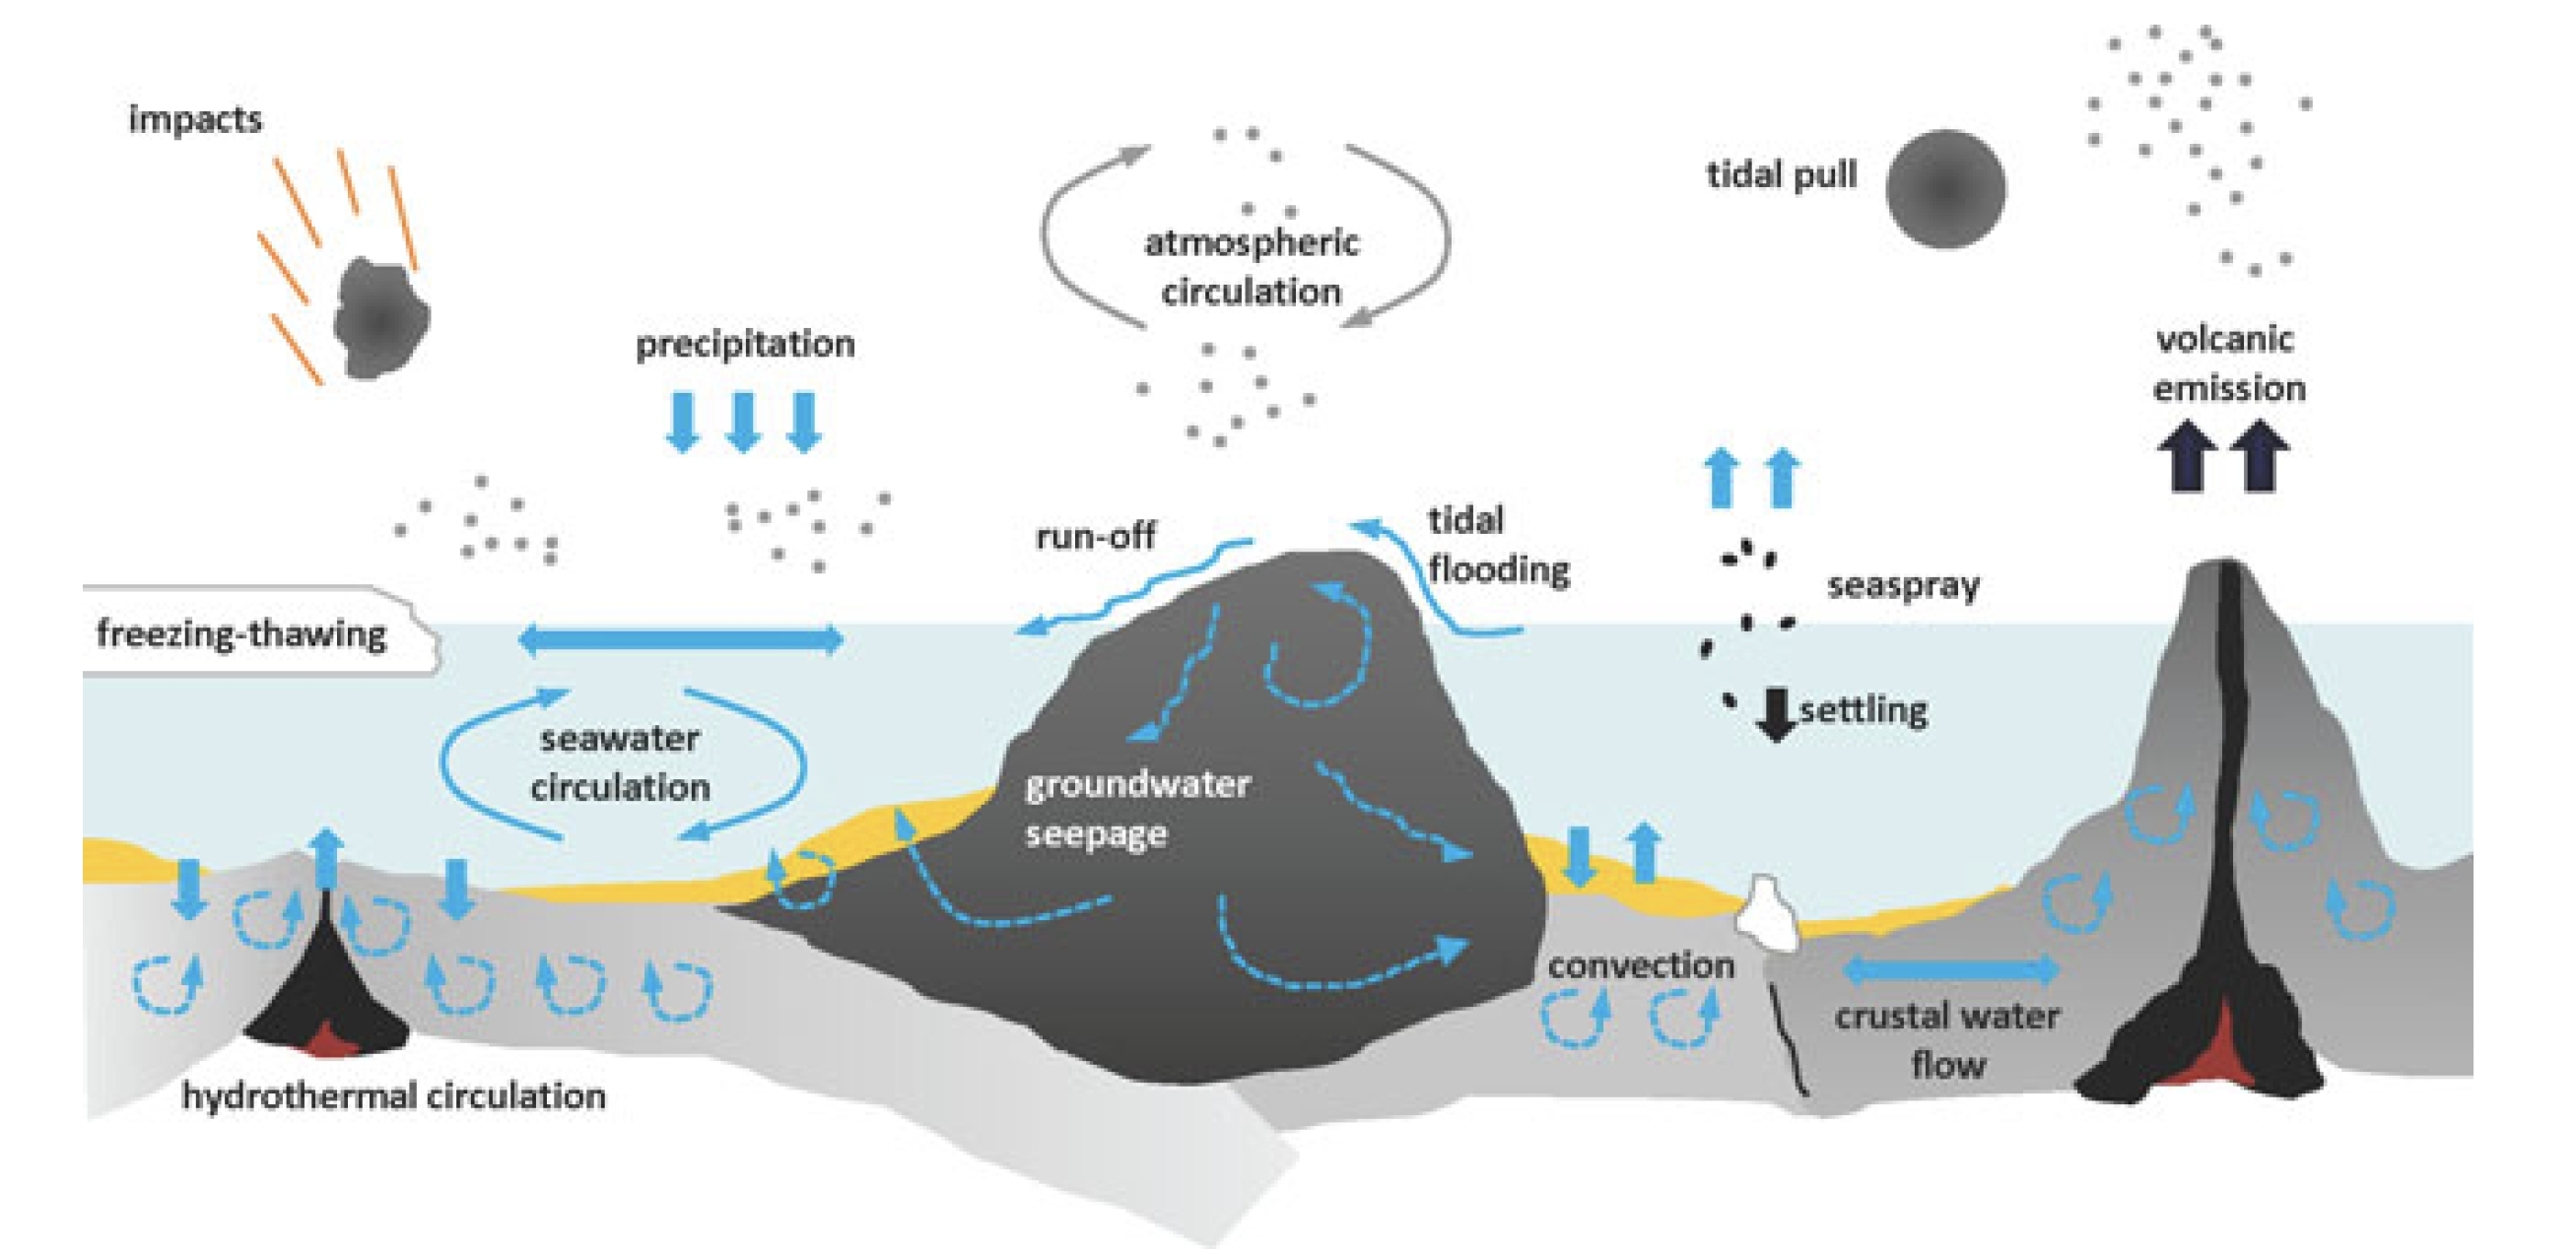
\includegraphics[width=0.9\textwidth]{MixingProcesses}
\end{figure}
Chemical reactions mixed by a variety of processes.

\begin{itemize}
	\item Tides
	\item Evaporation and aerosols
	\item Volcanic plumes
	\item Hydrothermal vents
\end{itemize}
  
  
\subsubsection{Geothermal systems}
\begin{figure}[h!]
	\caption{Geothermal systems \cite{damer2016field}}
	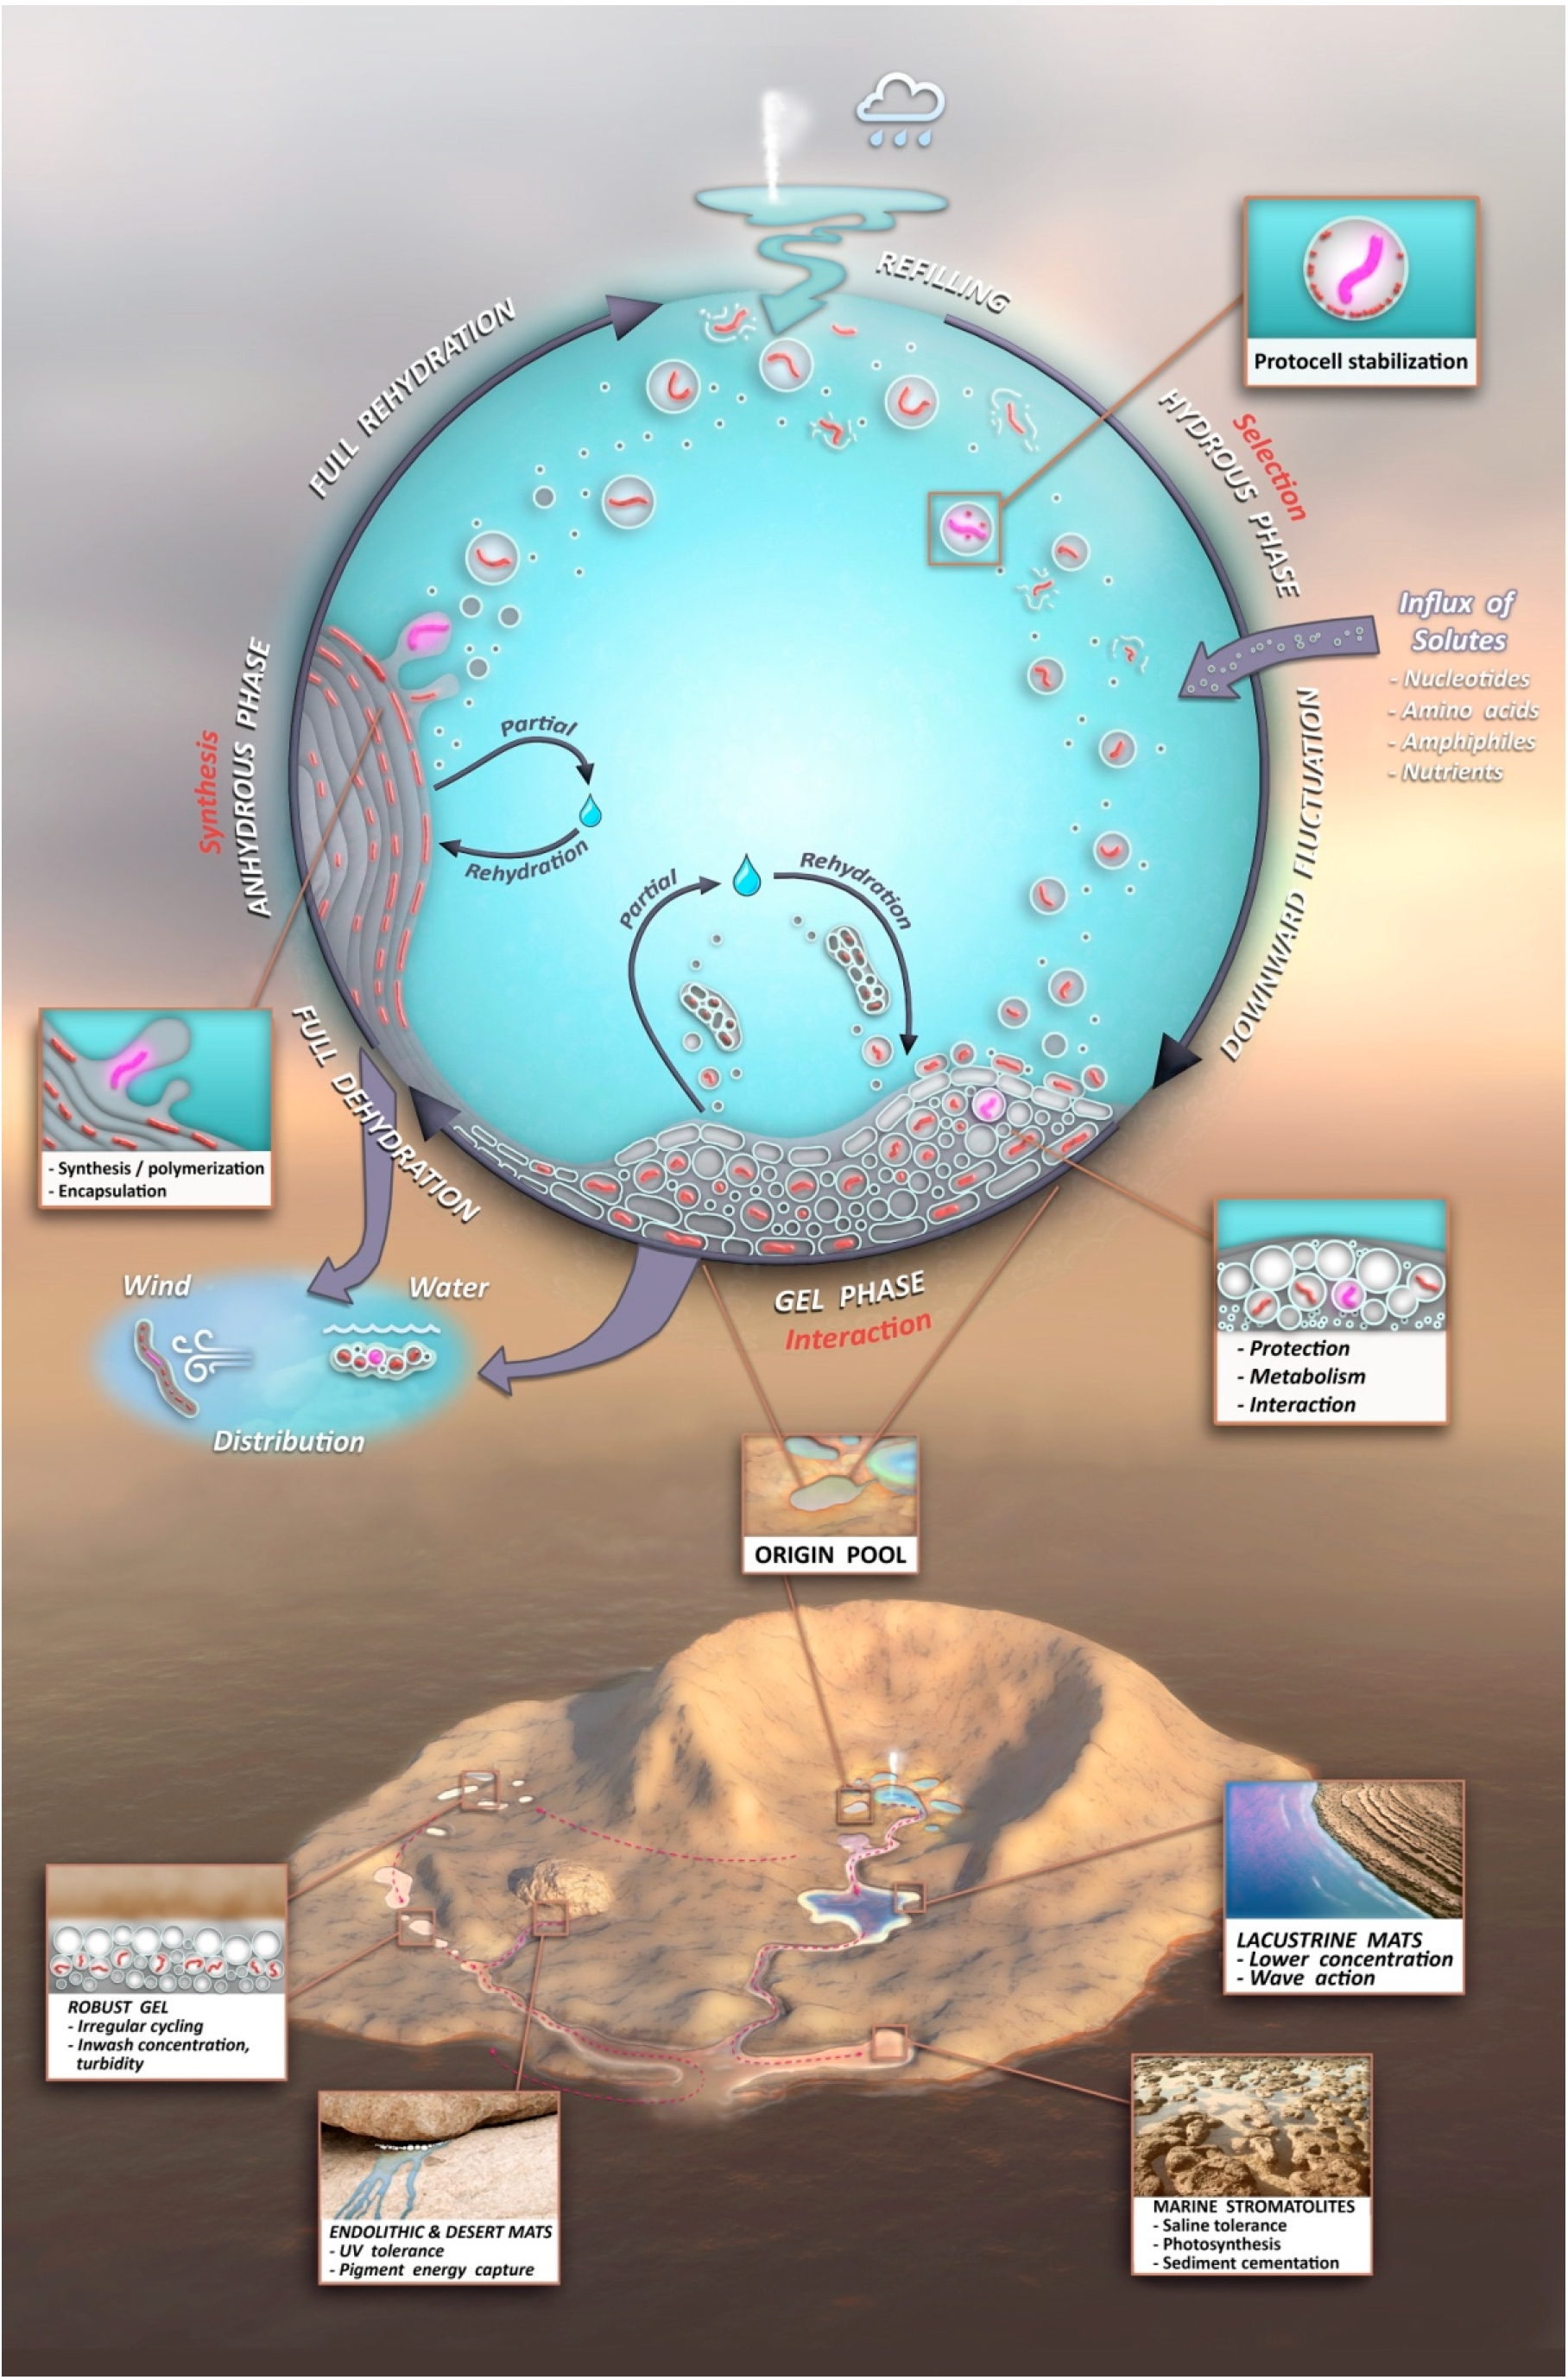
\includegraphics[width=0.9\textwidth]{GeothermalSystems}
\end{figure}

\begin{itemize}
	\item Provide high 	temperature, high
	pressure, reduced	reaction products
	\item Fresh water from 	precipitation
	\item Diversity of mineral	surfaces for ”nutrients” and catalysis
\end{itemize}

\subsubsection{Energy Sources}
\begin{itemize}
	\item Chemical Energy
	\begin{itemize}
		\item Reducing gases
		\item Radiation
		\item Minerals
	\end{itemize}
	\item Other Energy Sources
	\begin{itemize}
		\item Volcanic lightning
		\item UV-light
		\item High temperature
		\item Pressure
		\item Impacts
	\end{itemize}
\end{itemize}
Miller Urey. Maybe no methane, but CO2 to dive different mixture.

\begin{figure}[h!]
	\caption{Miller Urey \cite{miller1959organic}}
	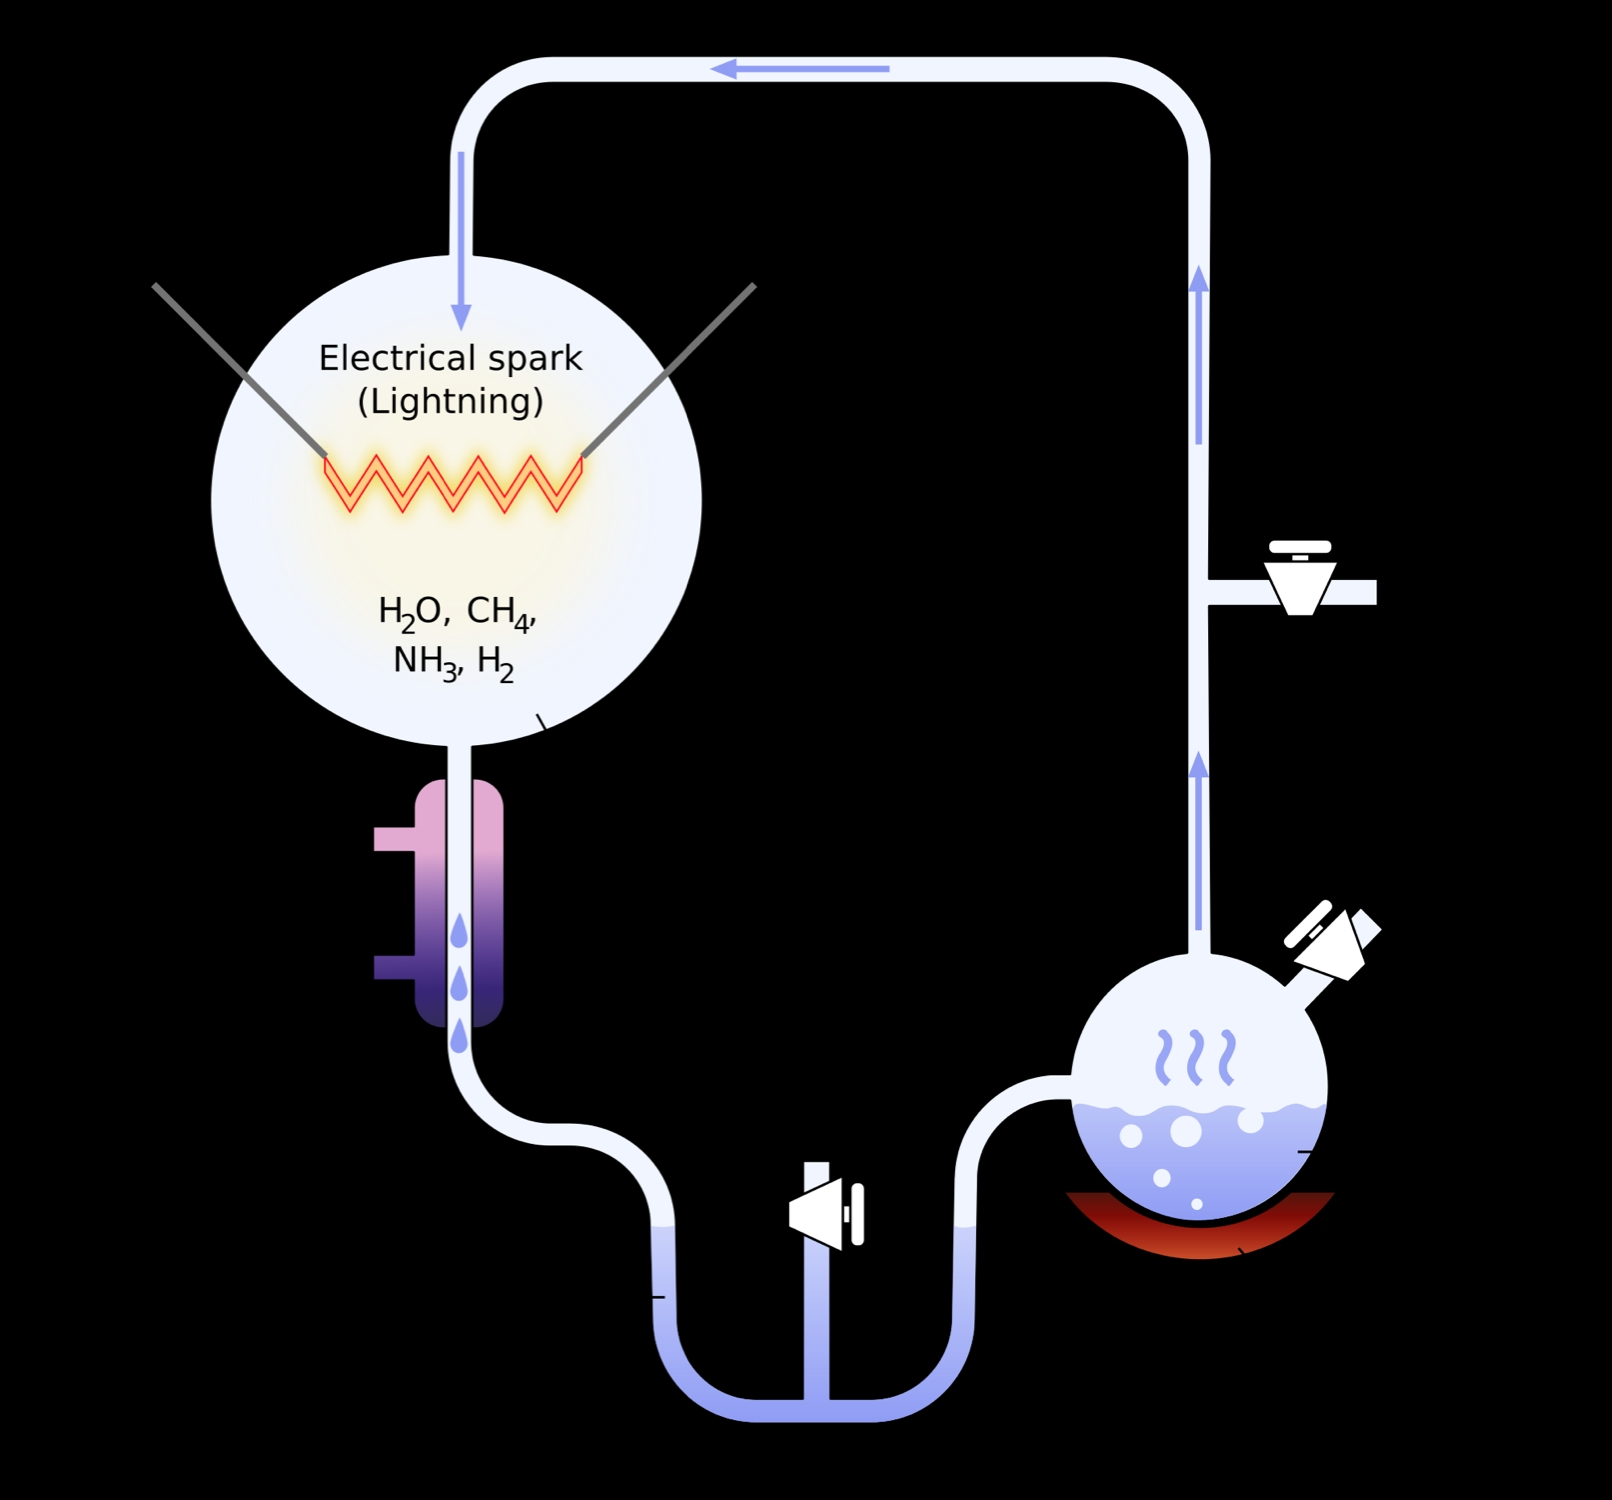
\includegraphics[width=0.45\textwidth]{MillerUrey1}
	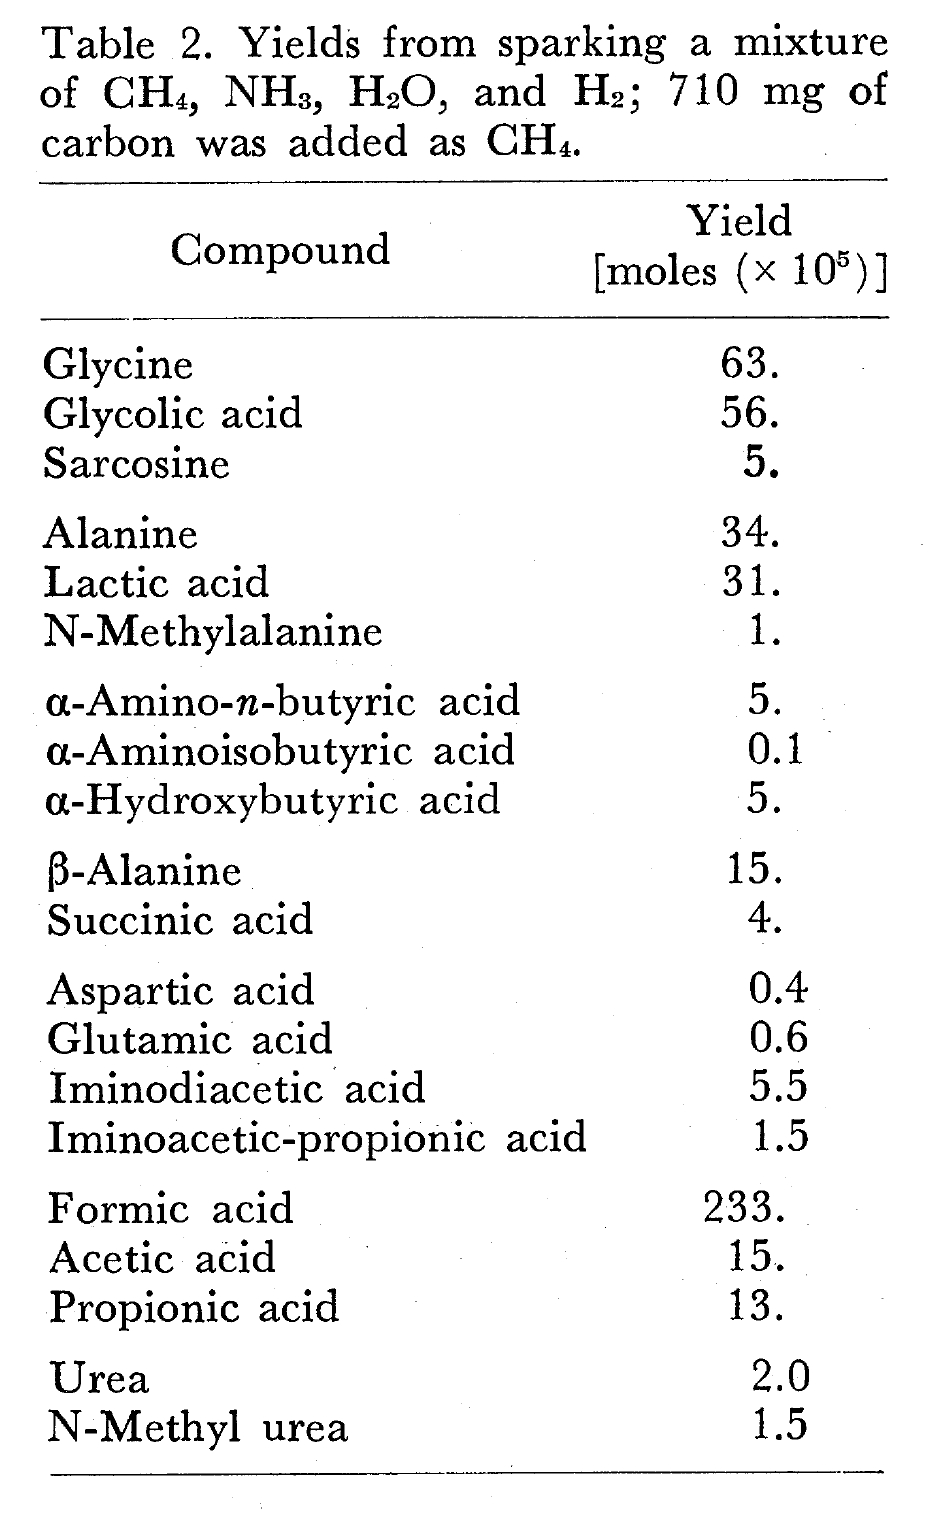
\includegraphics[width=0.45\textwidth]{MillerUrey2}
\end{figure}

Each meteorite has different chemical library

Enough material to jump start life

Bombardment

Samples and surface are (mostly) undisturbed
• Samples can be dated ( 40 Ar/ 39 Ar, 87 Rb/ 87 Sr, etc.)
• Craters can be counted
Lunar cratering rate anchors
the impact chronology for the
entire (inner) Solar System

Late Heavy Bombardment

\subsection{Likely Environments for Studying Origins of Life}

\begin{figure}[h!]
	\caption{Life probably started between 4.4 to 3.8 billion years ago (Ga) \cite{domagal2016astrobiology}}
	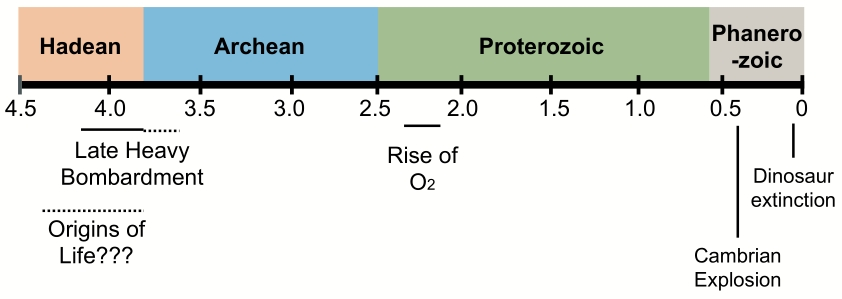
\includegraphics[width=0.9\textwidth]{LifeProbablyStarted}
\end{figure}

\begin{figure}[h!]
	\caption{Earth during the Hadean Eon was probably very inhospitable for life} 
	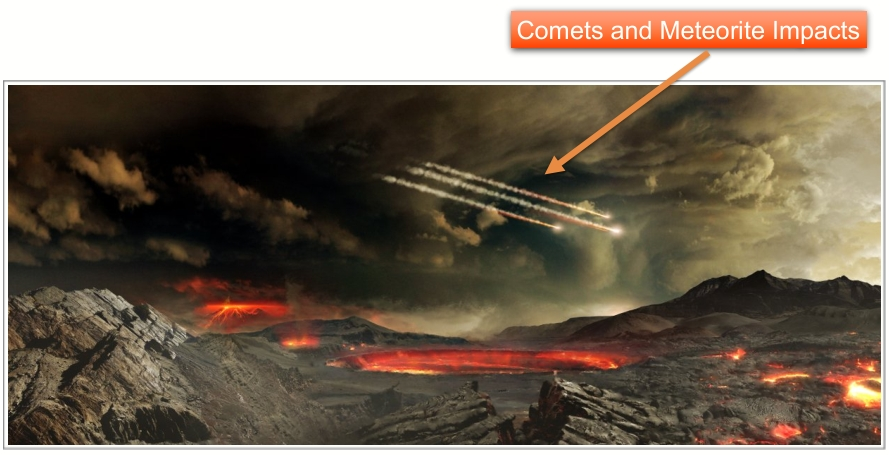
\includegraphics[width=0.9\textwidth]{HadeanInhospitable}
\end{figure}
 Magma Oceans formed because of:
\begin{itemize}
	\item Comets and meteorite impacts
	\item Tidal heating (moon/Earth)
	\item Core formation (plate tectonics)
\end{itemize}

Plate tectonics helped make the early Earth environment favorable for life

Global oceans probably covered the surface of the Earth by the Archean Eon



\begin{figure}[h!]
	\caption{Life took hold on Earth during the Archean Eon} 
		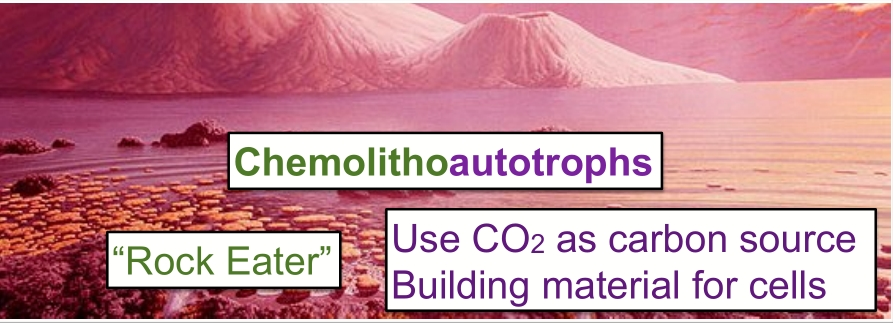
\includegraphics[width=0.9\textwidth]{Chemolithoautotrophs}
	\end{figure}

The first likely signs of life in the rock record dates back to 3.5 to 3.3 Ga

\subsection{Chemistry and The Origins of Life}

Tar problem: Biomolecules plus heat and time = black sludge.

\begin{itemize}
	\item What molecules can be and are created without life?
	\item How can these molecules be made to react in a life like manner?
	\item How can formation of wasteful byproducts like	tars be prevented?
\end{itemize}
\subsection{Why Nature Chose Phosphates}

\begin{itemize}
	\item Structural
	\begin{itemize}
		\item Nucleic Acid Backbones (Figure \ref{fig:PhosphoDiesterBond}-\ref{fig:PhosphoDiesterBond3})
		\item Phospholipid Bilayers (Figure \ref{fig:PhosphoLipid1}-\ref{fig:PhosphoLipid3})
	\end{itemize}

	\item Physical\begin{itemize}
		\item Compartmentalization
		\item Signaling
	\end{itemize}
	\item Chemical
	\begin{itemize}
		\item Energy
		\item Activation
	\end{itemize}
\end{itemize}

\begin{figure}[H]
	\caption{Nucleic Acid Backbones}
	\label{fig:three graphs}
	\begin{subfigure}[b]{0.45\textwidth}
		\centering
		\caption{Phospho Diester Bond}\label{fig:PhosphoDiesterBond} 
		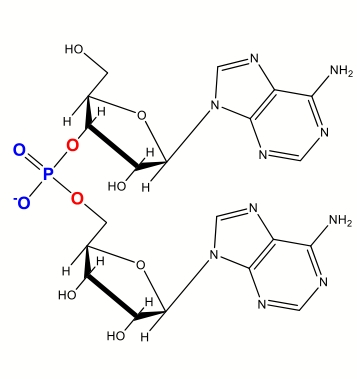
\includegraphics[width=\textwidth]{PhosphoDiesterBond}
	\end{subfigure}
	\begin{subfigure}[b]{0.45\textwidth}
		\centering
		\caption{Repels negatively charged nucleophiles which might break bond, so very stable}\label{fig:PhosphoDiesterBond1} 
		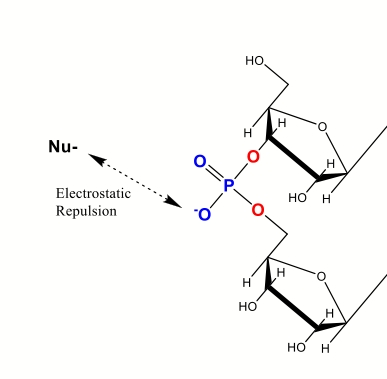
\includegraphics[width=\textwidth]{PhosphoDiesterBond1}
	\end{subfigure}
	\begin{subfigure}[b]{0.45\textwidth}
		\centering
		\caption{Bond is tunable if we need to react}\label{fig:PhosphoDiesterBond2} 
		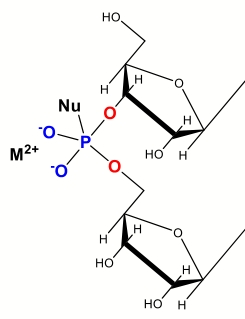
\includegraphics[width=\textwidth]{PhosphoDiesterBond2}
	\end{subfigure}
	\begin{subfigure}[b]{0.45\textwidth}
		\centering
		\caption{Repulsion keeps DNA soluble and prevents collapse}\label{fig:PhosphoDiesterBond3} 
		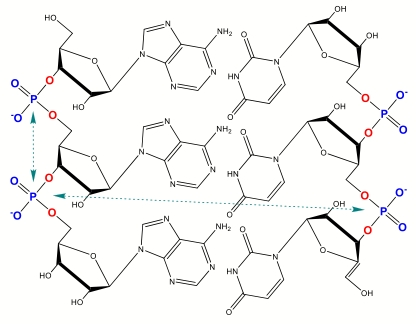
\includegraphics[width=\textwidth]{PhosphoDiesterBond3}
	\end{subfigure}
	
\end{figure}
\begin{figure}[H]
	\caption{Phospholipids}\label{fig:PhosphoLipids}
	
	\begin{subfigure}[b]{0.45\textwidth}
		\centering
		\caption{Phospho Diester Bond}\label{fig:PhosphoLipid1} 
		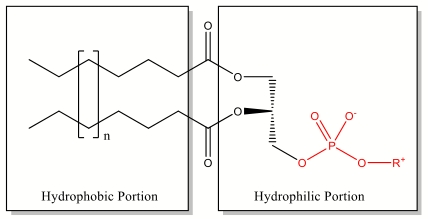
\includegraphics[width=\textwidth]{PhosphoLipid1}
	\end{subfigure}
	\begin{subfigure}[b]{0.45\textwidth}
		\centering
		\caption{Repels negatively charged nucleophiles which might break bond, so very stable}\label{fig:PhosphoLipid2} 
		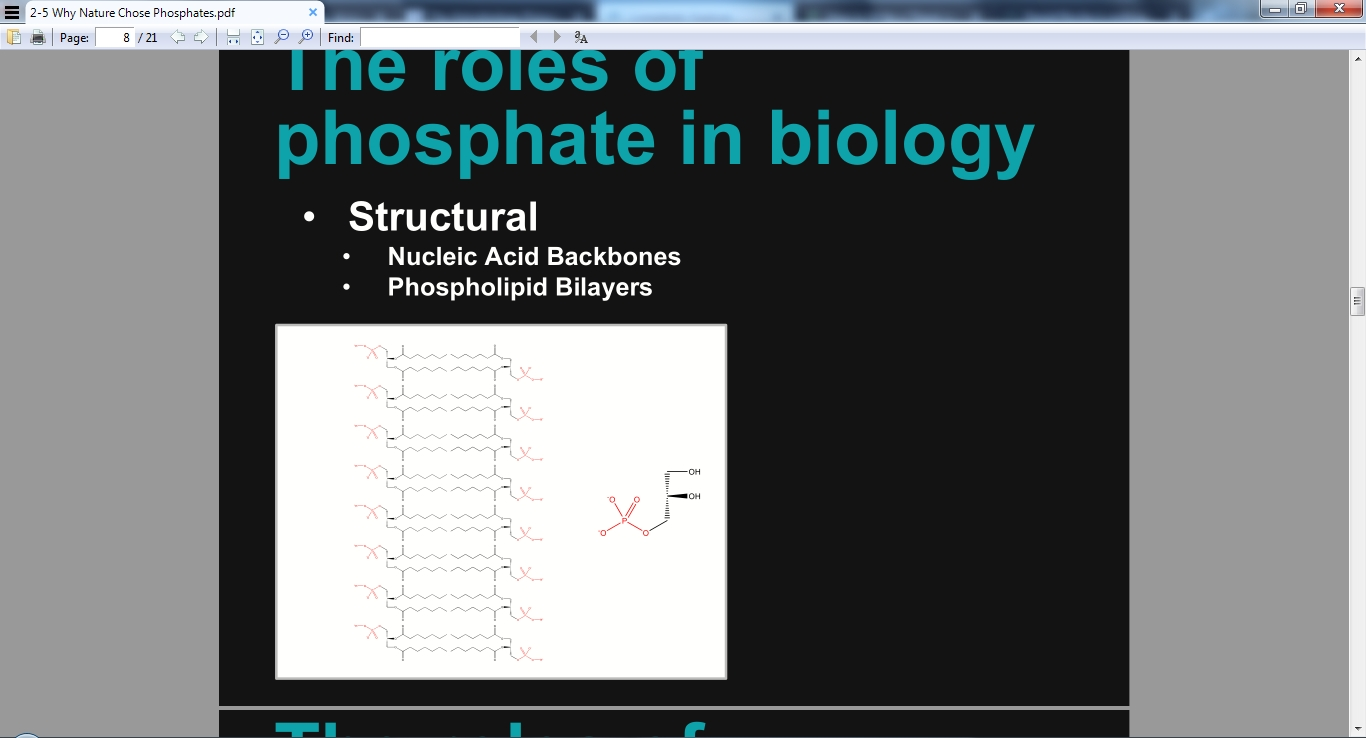
\includegraphics[width=\textwidth]{PhosphoLipid2}
	\end{subfigure}
	
	\begin{subfigure}[b]{0.45\textwidth}
		\centering
		\caption{Repulsion keeps DNA soluble and prevents collapse}\label{fig:PhosphoLipid3} 
		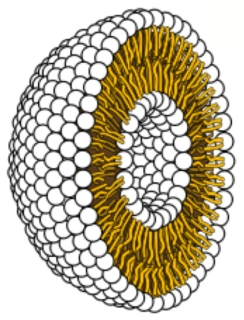
\includegraphics[width=\textwidth]{PhosphoLipid3}
	\end{subfigure}
	
\end{figure}

Why wouldn't you use phosphate?

\begin{itemize}
	\item Scarce
	\item Insoluble, unreactive
	\item No polyphosphate minerals
	\item One pyrophosphate mineral
	\item Limited geochemical production of reactive forms
\end{itemize}
Open Questions

\begin{itemize}
	\item When did life begin to use 	phosphate?
	\item If not at the very beginning, what 	came before?
	\item Where did early phosphate come 	from?
\end{itemize}
Backbone of nucleic acids: strong bond, tunable

\subsection{Why Water, Why Carbon}
\subsection{Macromolecules}
\subsection{Chemical Cycles and Chaos}
\subsection{Fossil or Not?}

\section{Chemical Commonalities}

\section{Early Life}

\section{Evolution}

\section{Astrobiology \& General Theories of Life}

\bibliographystyle{unsrt}
\bibliography{origins}

\end{document}
